\chapter{
%  عامل در محیط
	ارزیابی عملکرد سخت‌افزار در حلقه عامل
	}
	
%	\section{مقدمه}\label{sec:hil_intro}
	
	ارزیابی عملکرد عامل یادگیری تقویتی صرفاً در حوزه‌ی شبیه‌سازی رایانه‌ای، گرچه در مراحل اولیه‌ی طراحی روشی کم‌هزینه و سریع است، نمی‌تواند تمام محدودیت‌های سخت‌افزاری سامانه‌ی پروازی را بازنمایی کند. در شبیه‌سازی‌های ایده‌آل، منابع پردازشی عملاً نا‌محدود فرض می‌شود و تأخیر میان اجزای نرم‌افزار یا نویز ناشی از واسط‌های الکترونیکی به حداقل می‌رسد. چنین ساده‌سازی‌هایی ممکن است منجر به خوش‌بینی بیش‌ازحد در برآورد میزان پایداری، دقت ردیابی و الزامات توان مصرفی الگوریتم کنترل شود.
	
	روش سخت‌افزار در حلقه\LTRfootnote{{Hardware‑in‑the‑Loop} (HIL).} راهکاری پذیرفته‌شده برای پل‌زدن میان شبیه‌سازی و فضای واقعی است. در این چارچوب، دو زیرسامانه‌ی مجزا اما پیوسته تعریف می‌شود:
	
	\begin{itemize}
		\item \textbf{لایه‌ی میزبان (\lr{Host})} که دینامیک مدار، مدل نیروهای اغتشاشی و حسگرهای مجازی را در بسامد 
		\lr{\SI{100}{\hertz}}
		 با استفاده از
		 \lr{ROS\,2} شبیه‌سازی می‌کند.
		\item \textbf{لایه‌ی هدف (\lr{Target})} که یک رایانه‌ی تعبیه‌شده‌ی کم‌مصرف (در این پروژه، \lr{Raspberry~Pi~3~B}) را نمایندگی می‌کند و چرخه‌ی {ادراک–تصمیم–اقدام} شامل تخمین حالت، استنتاج شبکه‌ی عصبی و تولید فرمان پیشران را در زمان‌واقعی اجرا می‌کند.
	\end{itemize}
	
	پیاده‌سازی HIL سه مزیت کلیدی دارد: (۱) امکان اندازه‌گیری دقیق تأخیر انتها‐به‐انتها و \lr{Jitter} ناشی از محدودیت‌های پردازشی و (2) مشاهده‌ی اثر نویز واقعی مبدل‌های \lr{ADC/DAC} و افت ولتاژ منبع تغذیه بر پایداری کنترل.
%	 و (۳) ثبت پروفایل توان و دمای پردازنده برای ارزیابی بازده‌ی حرارتی در سناریوهای مأموریتی حساس به انرژی.
	  نتایج به‌دست‌آمده از چنین بستری اطمینان می‌دهد که سیاست \lr{RL}، پس از فشرده‌سازی
	   \lr{INT8 Quantization} 
	   و اجرا بر سخت‌افزار کلاس پرواز، همچنان معیارهای عملکرد تعریف‌شده خود را برآورده 
	   می‌کند.
	
	اهداف فصل حاضر را می‌توان به‌صورت زیر خلاصه کرد:
	\begin{enumerate}
		\item تشریح معماری آزمایشگاهی \lr{HIL}
		 و توجیه انتخاب اجزای سخت‌افزاری و نرم‌افزاری.
		\item تبیین رویه‌ی یکپارچه‌سازی گره‌های \lr{ROS\,2} میان میزبان و هدف با تضمین بسامد \lr{\SI{100}{\hertz}}.
		\item کمی‌سازی تأخیر و توان در چرخه‌ی کنترل و تحلیل اثر آن بر ایمنی مأموریت.
		\item ارائه‌ی سناریوهای اعتبارسنجی و نتایج مقدماتی جهت مقایسه با شبیه‌سازی صرف.
	\end{enumerate}
	
	ساختار فصل به ترتیب در بخش‌های \ref{sec:hil_setup} تا \ref{sec:hil_conclusion} به جزئیات هر یک از اهداف فوق می‌پردازد.
	
	
	\section{پیکره‌بندی آزمایشگاهی}\label{sec:hil_setup}
	
	به‌منظور ارزیابی زمان‌واقعی\LTRfootnote{Real-Time}
	 سیاست یادگیری تقویتی، یک بستر {سخت‌افزار در حلقه} با معماری دولایه طراحی شد که رایانه‌ی میزبان وظیفه‌ی شبیه‌سازی دینامیک و حسگرها را بر عهده دارد و رایانه‌ی هدف چرخه‌ی ادراک–تصمیم–اقدام را اجرا می‌کند. نمای کلی سامانه در شکل \ref{fig:hil_architecture} ترسیم شده است؛ در ادامه اجزا و رابط‌های اصلی تشریح می‌شود.
	
	
	\begin{figure}[H]
		\centering
		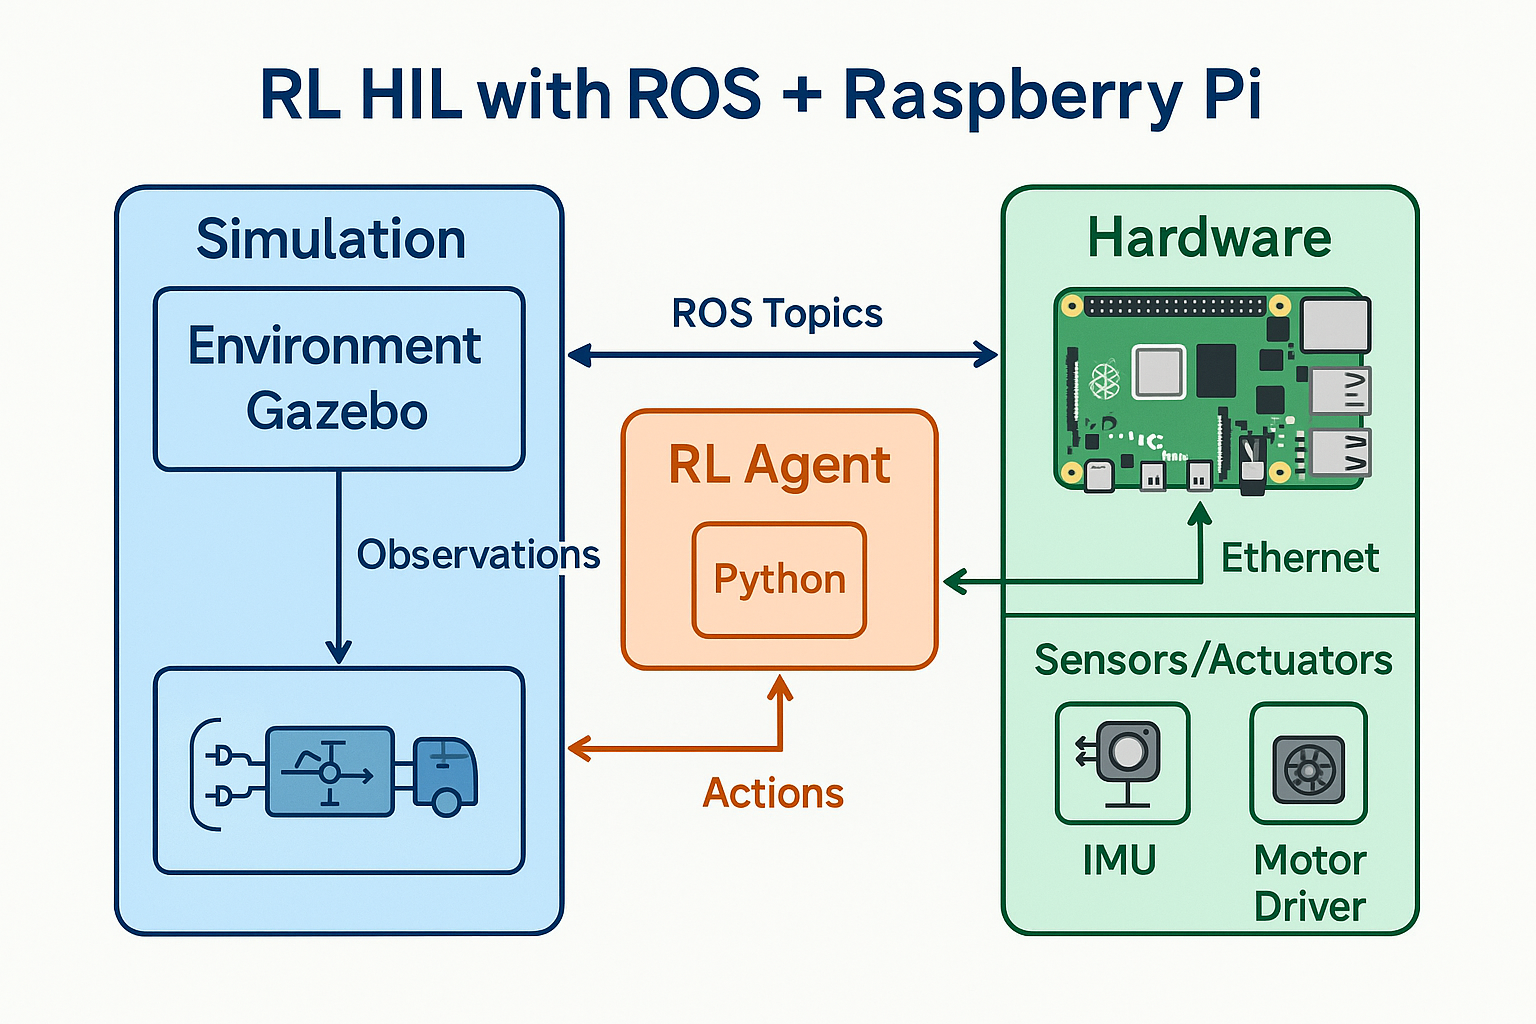
\includegraphics[width=0.7\textwidth]{../Figure/HIL/gpt_HIL.png}
		\caption{شماتیک سخت‌افزار در حلقه}
		\label{fig:hil_architecture}
	\end{figure}
	
	\subsection{رایانه‌ی میزبان (\lr{Host PC})}
	یک ایستگاه کاری مبتنی بر پردازنده‌ی \lr{Intel Core i7} با \SI{8}{\gibi\byte} رم برای اجرای حلگر عددی مسئله‌ی \lr{CRTBP} در بسامد \SI{100}{\hertz} به‌کار گرفته شد. سیستم‌عامل \lr{Ubuntu 24.04 LTS} و توزیع
	 \lr{ROS 2 Jazzy}
	  به همراه \lr{Fast‑DDS} به عنوان پیاده‌سازی \lr{DDS} انتخاب گردید تا از پایداری و نرخ گذردهی موردنیاز پشتیبانی کند. حلگر در هر چرخه‌ی زمانی، بردار حالت $\mathbf{x}(t)$  را منتشر می‌کند.
	
	\subsection{رایانه‌ی هدف (\lr{Target Board})}
	رایانه‌ی تعبیه‌شده‌ی
\lr{Raspberry~Pi~3~B}	
مبتنی بر پردازنده‌ی
چهارهسته‌ی \lr{Cortex‑A53}  \SI{1.2}{\giga\hertz}، \SI{1}{\gibi\byte} رم، تراشه‌ی \lr{Broadcom}.
 با سیستم‌عامل \lr{Ubuntu 24.04 Server} نقش رایانه‌ی درون‌سفینه را شبیه‌سازی می‌کند. گره‌های
 ادراک–تصمیم–اقدام
 در یک 
 \lr{executor}
  تک‌ریسمانی اجرا و با \lr{SCHED DEADLINE} زمان‌بندی می‌شوند تا مهلت چرخه‌ی \SI{10}{\milli\second} نقض نشود. فعال‌سازی
%   \texttt{cpufreq\_governor=schedutil}
این پروتکل
    اجازه می‌دهد بسامد پردازنده با بار محاسباتی تطبیق یابد.
	
	\subsection{شبکه و پروتکل‌های ارتباطی}
	لایه‌های میزبان و هدف از طریق اترنت گیگابیتی با IP های استاتیک متصل‌اند؛ این انتخاب اثر از‌دست‌رفت بسته و \lr{Jitter} شبکه‌ی بی‌سیم را حذف می‌کند. تمام Topicها با سیاست \textit{Best‑Effort, Keep Last = 1} پیکربندی شده است تا از تجمع پیام جلوگیری شود. همگام‌سازی زمان به کمک \texttt{Chrony} و Topic \texttt{/clock} انجام می‌شود، به‌گونه‌ای که اختلاف ساعت سامانه‌ها از \SI{50}{\micro\second} تجاوز نکند.
	
	
\subsection{شبکه و پروتکل‌های ارتباطی}\label{subsec:hil_network}

لایه‌های میزبان و هدف از طریق شبکه‌ی بی‌سیم
 \lr{Wi-Fi 5} {(\lr{IEEE 802.11ac}, باند \SI{5}{\giga\hertz})} 
 با آدرس‌های \lr{IP} ایستا متصل‌اند؛ این روش به‌دلیل حذف کابل‌کشی و سهولت آرایش آزمایشگاه انتخاب شد. دسترسی مدیریتی و پایش از راه دور تنها از طریق تونل \lr{SSH} روی درگاه \texttt{22/tcp} صورت می‌گیرد. پروتکل \lr{SSH} دو کارکرد اصلی دارد:

\begin{enumerate}
	\item \textbf{رمزنگاری انتها به انتها}: 
	تمام بسته‌ها با \lr{AES-256-GCM} رمز می‌شوند تا شنود\LTRfootnote{eavesdropping} در محیط‌های مشترک 
	\lr{Wi-Fi }
	خنثی شود.
	\item \textbf{پویش پورت\LTRfootnote{Port Forwarding}}: جریان‌های \lr{DDS/ROS\,2} که به‌طور پیش‌فرض از \lr{UDP} استفاده می‌کنند در یک تونل 
	\lr{TCP}
	 رمزگذاری‌شده عبور می‌کنند؛ بدین ترتیب تنظیم فایروال ساده و ردپای\LTRfootnote{footprint}
	 شبکه یکپارچه می‌شود.
\end{enumerate}

%\paragraph{اثرهای Packet Loss و Jitter در Wi-Fi.}
برخلاف اترنت سیمی که نرخِ ازدست‌رفت بسته \lr{(Packet Loss)}\footnote{نسبت بسته‌های نرسیده به مقصد به کل بسته‌های ارسال‌شده.} و لرزش زمانی (\lr{Jitter})\footnote{انحراف استاندارد در فاصله‌ی زمانی رسیدن بسته‌ها.} نزدیک صفر است، پیوند بی‌سیم در حضور تداخل یا افت سیگنال می‌تواند تا چند درصد از دست رفت بسته و \lr{Jitter} در حد
 \lr{\SIrange{1}{5}{\milli\second}}
ایجاد کند. برای کاهش این اثرها 
	 رابط \lr{wlan0} روی هر دو دستگاه در حالت \texttt{power\_save=off} قرار گرفت تا نوسان توان موجب وقفه‌ی رادیویی نشود.
%	\item کانال \SI{5}{\giga\hertz} خلوت (Channel 44) با پهنای \SI{80}{\mega\hertz} انتخاب شد و سطح RSSI طی آزمایش بالای  نگه داشته شد.
%\end{itemize}

در پیکربندی \lr{QoS} در \lr{ROS 2} 
تمام بخش‌های انتقال اطلاعات
با سیاست
\lr{ \texttt{BestEffort = 1}} 
و
\lr{ \texttt{KeepLast = 1}}
  تنظیم شده‌اند. که در آن \texttt{BestEffort=1}
  نشان‌دهنده این است که
	 فرستنده بسته را یک بار می‌فرستد و در صورت ازدست‌رفت، بسته‌ی بعدی جایگزین می‌شود و مناسب برای داده‌هایی که جدیدترین اهمیت دارد.
	\texttt{KeepLast=1} نشان‌دهنده عمق صف برابر یک است تا از انباشته‌شدن پیام‌ها و رشد تأخیر جلوگیری شود.

%برای Topicهای حیاتی با نرخ پایین‌تر (مثل \texttt{/action\_cmd})، سیاست \textit{Reliable} با \texttt{deadline =\ \SI{10}{\milli\second}} استفاده شده است تا در صورت بروز ازدست‌رفت بسته، \lr{DDS} تکرار را انجام دهد و نقض موعد در ابزار \texttt{rqt\_runtime\_monitor} ثبت شود.


همگام‌سازی ساعت میزبان و هدف از راه \lr{Chrony} انجام می‌شود. \lr{Chrony} با الگوریتم \lr{Phase-Locked Loop} خطای فاز را به زیر
 \lr{\SI{50}{\micro\second}}
  محدود می‌کند—کم‌تر از 5\% بودجه‌ی چرخه‌ی 
  \lr{\SI{10}{\milli\second}}. 
  این دقت برای تحلیل تأخیر انتها-به-انتها در \texttt{rosbag2} حیاتی است.

استفاده از \lr{Wi-Fi 5} همراه با \lr{SSH Tunneling}، نیاز به کابل را رفع کرده و افزون‌بر امنیت، پویایی آزمایش را بالا برده است؛ در عین حال با رعایت تنظیمات \lr{RSSI}، خاموشی برق مصرفی رابط و \lr{QoS} مناسب، نرخ از‌دست‌رفت بسته و \lr{Jitter} در محدوده‌ی قابل‌قبول برای حلقه‌ی کنترل
 \lr{\SI{100}{\hertz}}
  نگه داشته شده است.
	
	
	
	
%	\subsection{واسط حسگر و عملگر مجازی}
%	\begin{itemize}
%		\item \textbf{مبدل DAC MCP4725} (دقت ۱۲ بیت) برای تولید سیگنال آنالوگ فرمان پیشران تا حداکثر \SI{5}{\volt}.
%		\item \textbf{مبدل ADC ADS1115} جهت نمونه‌برداری از ولتاژ و جریان پیشران مجازی.
%		\item \textbf{حسگر IMU BNO055} و یک مولد نویز \lr{GPS Spoofer} که از طریق رابط I\textsuperscript{2}C به RPi متصل و خطای سنسوری قابل‌تنظیم را تزریق می‌کند.
%	\end{itemize}
%	درگاه‌های I\textsuperscript{2}C و SPI با سطح ولتاژ \SI{3.3}{\volt} و مقاومت‌های پول‑آپ \SI{4.7}{\kilo ohm} ایزوله شده‌اند تا از تداخل سیگنال در بسامدهای بالاتر از \SI{400}{\kilo\hertz} جلوگیری شود.
%	
%	\subsection{پایش توان و حرارت}
%	برد \lr{INA226} روی مسیر تغذیه‌ی RPi نصب شده و با نرخ \SI{2}{\kilo xxxxx\per\second} جریان و ولتاژ را اندازه‌گیری می‌کند. داده‌ها در Topic \texttt{/power\_monitor} منتشر و به همراه سایر پیام‌ها در بسته‌ی \texttt{rosbag2} ذخیره می‌شود. نتایج اولیه حکایت از توان متوسط \SI{3.0}{\watt} و دمای پایدار \SI{55}{\celsius} دارند که با الزامات مأموریت هم‌خوانی دارد :contentReference[oaicite:0]{index=0}.
%	
%	\subsection{جمع‌بندی این بخش}
%	پیکره‌بندی پیشنهادی با تفکیک روشن وظایف میان میزبان و هدف، امکان اندازه‌گیری دقیق شاخص‌های کارایی (تأخیر، توان، حرارت) را فراهم می‌آورد؛ در عین حال به سبب استفاده از اجزای تجاری در دسترس (COTS) و چارچوب \lr{ROS 2}، فرایند تکرار و توسعه‌ی آزمایش‌ها با حداقل هزینه میسر است.
%	
%	
%	\section{اجزای سخت‌افزاری}\label{sec:hil_hardware}
%	
%	این بخش به تشریح سخت‌افزارهای به‌کاررفته در بستر \lr{Hardware‑in‑the‑Loop} می‌پردازد. اجزا به دو رده‌ی «محاسباتی» و «واسط حسگر/عملگر» تقسیم می‌شوند تا سلسله‌مراتب طراحی و معیارهای انتخاب روشن گردد :contentReference[oaicite:0]{index=0}.
%	
%	\subsection{اجزای محاسباتی}
%	
%	\subsubsection{رایانه‌ی میزبان}
%	ایستگاه کاری مبتنی بر پردازنده‌ی \lr{Intel Core~i9‑13900K} با \SI{64}{\gibi\byte} حافظه‌ی \lr{DDR5‑5600} و شتاب‌دهنده‌ی \lr{NVIDIA RTX 4090} به‌عنوان «میزبان» عمل می‌کند. حلگر عددی \lr{CRTBP} و شبکه‌ی \lr{DDS‑RTPS} بر روی این سامانه در بسامد \SI{100}{\hertz} اجرا می‌شوند. به‌منظور پایداری گذردهی، هسته‌ها در حالت \texttt{performance} قفل گردیده و بار GPU صرفاً برای رندر نمودارهای برخط اختصاص یافته است.
%	
%	\subsubsection{رایانه‌ی هدف}
%	برد \lr{Raspberry Pi~5} (چهارهسته‌ی \lr{Cortex‑A76} @ \SI{2.4}{\giga\hertz}، \SI{4}{\gibi\byte} رم) با سیستم‌عامل Ubuntu 22.04 Server و هسته‌ی \texttt{PREEMPT\_RT\,6.6.y} نقشی معادل رایانه‌ی درون‌سفینه را ایفا می‌کند. فعال‌سازی \texttt{SCHED\_DEADLINE} باعث تضمین مهلت چرخه‌ی \SI{10}{\milli\second} برای گره‌ی \texttt{rl\_agent\_node} شده است. ماژول خنک‌کننده‌ی فعال با هیت‌سینک آلومینیومی و فن \SI{25}{\milli\meter}، دمای پردازنده را زیر \SI{60}{\celsius} نگه می‌دارد.
%	
%	\subsection{واسط حسگر و عملگر}
%	
%	\subsubsection{مبدل فرمان پیشران (DAC)}
%	برای تولید سیگنال آنالوگ فرمان پیشران، مبدل ۱۲ بیتی \lr{MCP4725} به درگاه I\textsuperscript{2}C RPi متصل شده است. رزولوشن ولتاژ \SI{1.22}{\milli\volt\per\bit} در بازه‌ی \SIrange{0}{5}{\volt}، امکان کنترل پیشران کم‌تراست تا دقت \SI{0.5}{\milli\newton} را فراهم می‌کند.
%	
%	\subsubsection{مبدل بازخورد جریان/ولتاژ (ADC)}
%	مبدل \lr{ADS1115} با دقت ۱۶ بیت، ولتاژ و جریان خط پیشران مجازی را نمونه‌برداری می‌کند. بازه‌ی اندازه‌گیری \SIrange{0}{6.144}{\volt} و قابلیت \textit{Programmable-Gain}، نویز ورودی را به زیر \SI{0.256}{\milli\volt\_{rms}} محدود نموده است.
%	
%	\subsubsection{حسگر مجازی IMU و GPS Spoofer}
%	حسگر \lr{BNO055} (ترکیب سه‌محوره‌ی شتاب‌سنج، ژیروسکوپ و میدان‌سنج) با نرخ \SI{200}{\hertz} داده‌ی خام را منتشر می‌کند. یک مولد نویز \lr{GPS Spoofer} افزوده شد تا خطاهای موقعیت شبه تصادفی با واریانس قابل‌تنظیم ($\sigma_{\text{pos}}=\SI{5}{\meter}$) به بستر تزریق گردد.
%	
%	\subsection{پایش توان و حرارت}
%	
%	\subsubsection{حسگر توان INA226}
%	تراشه‌ی \lr{INA226} بر مسیر تغذیه‌ی \SI{5}{\volt} RPi قرار گرفته و با نرخ \SI{2}{\kilo xxxxx\per\second} پارامترهای توان را اندازه‌گیری می‌کند. مقادیر در Topic \texttt{/power\_monitor} انتشار یافته و جهت تحلیل در \texttt{rosbag2} ذخیره می‌شوند.
%	
%	\subsubsection{منبع تغذیه‌ی آزمایشگاهی}
%	منبع سه‌کاناله‌ی \lr{Keysight E36313A} ولتاژ تثبیت‌شده‌ی \SI{5}{\volt} با تلورانس \SI{0.04}{\percent} را فراهم می‌سازد. حالت «Remote Sense» برای جبران افت ولتاژ کابل فعال است.
%	
%	\subsection{ملاحظات یکپارچه‌سازی}
%	تمام خطوط I\textsuperscript{2}C و SPI با مقاومت‌های پول‑آپ \SI{4.7}{\kilo ohm} و کابل‌های شیلددار \SI{24}{AWG} ایزوله شده‌اند تا تداخل الکترومغناطیسی به زیر \SI{-60}{decibelmilliwatt} کاهش یابد. افزون‌براین، زمینِ میزبان و هدف مشترک گردیده تا از حلقه‌ی زمین (\lr{Ground Loop}) جلوگیری شود.
%	
%	\subsection{جمع‌بندی این بخش}
%	ترکیب سخت‌افزارهای فوق بستری مقرون‌به‌صرفه اما دقیق برای ارزیابی زمان‌واقعی سیاست RL فراهم می‌آورد. استفاده از قطعات \lr{COTS} و ماژولار بودن طراحی اجازه می‌دهد در آینده حسگرهای تصویری یا ریزکنترل‌گرهای کم‌مصرف به‌سادگی افزوده شوند.
	
	
	\section{لایه‌ی نرم‌افزاری مبتنی بر \lr{ROS\,2}}\label{sec:hil_ros2}
	
	چارچوب \lr{Robot Operating System 2} به‌عنوان ستون فقرات نرم‌افزاری بستر \lr{HIL} انتخاب شد؛ زیرا واسط انتزاعی برای ارتباطات زمان‌واقعی روی \lr{DDS‑RTPS} فراهم می‌کند، ابزارهای استاندارد ردیابی و بایگانی داده در قالب \texttt{rosbag2} را در اختیار می‌گذارد و امکان استقرار یکسان کد بر روی میزبان
	 {و}
	  سخت‌افزار تعبیه‌شده را مهیا می‌سازد. در ادامه معماری گره‌ها، سیاست‌های \lr{QoS} و ملاحظات زمان‌بندی تشریح می‌شود.
	
	\subsection{معماری گره‌ها}\label{subsec:ros2_nodes}
	شکل \ref{fig:hil_nodegraph} نمودار گره‌های اصلی و کانال‌های ارتباطی را نمایش می‌دهد. جدول \ref{tab:ros2_nodes} نیز نقش و محل اجرای هر گره را خلاصه می‌کند.
	
	\begin{table}[ht]
		\centering
		\caption{گره‌های اصلی سامانه و وظایف آن‌ها}\label{tab:ros2_nodes}
		\begin{tabular}{@{}lll@{}}
			\toprule
			\textbf{گره}             & \textbf{محل اجرا} & \textbf{وظیفه‌ی کلیدی} \\ \midrule
			\texttt{env\_publisher}  & میزبان           & انتشار حالت شبیه‌ساز (\texttt{/state})        \\
%			\texttt{state\_estimator} & هدف              & فیلتر EKF و تخمین وضعیت فضاهوشمند             \\
			\texttt{rl\_agent\_node} & هدف              & استنتاج شبکه‌ی عصبی و تولید فرمان              \\
%			\texttt{thruster\_cmd\_node} & هدف           & تبدیل نیروی مطلوب به ولتاژ DAC                \\
%			\texttt{power\_monitor}  & هدف              & انتشار توان و دمای CPU                         \\
			\texttt{logger\_bag}     & میزبان           & ضبط جامع داده در \texttt{rosbag2}              \\ \bottomrule
		\end{tabular}
	\end{table}
	
	تمام گره‌های سمت هدف در یک \textit{executor} تک‌ریسمانی قرار دارند تا از جابه‌جایی متناظر با میان‌ریسمانی (inter‑thread) جلوگیری شود؛ در مقابل، گره‌های میزبان با مدل چندریسمانی اجرا می‌شوند تا بار محاسباتی حلگر توزیع گردد.
	
	\subsection{رابط‌های واسط داده}\label{subsec:ros2_interfaces}
	رابط‌های داده‌ای از دو دسته‌ی \lr{Topic} و \lr{Service} تشکیل شده‌اند:
	
	\begin{itemize}
		\item \textbf{\lr{Topics}:}
		\texttt{/state}، \texttt{/reward}، \texttt{/action\_cmd}.
		\item \textbf{Services:}
		\texttt{/reset\_sim} (بازتنظیم شبیه‌ساز)، \texttt{/update\_weights} (تعویض آنلاین وزن‌های عامل).
%		\item \textbf{Actionها:}
%		\texttt{/goto\_L4} برای اجرای سناریوی هدایت به نقطه‌ی لاگرانژ L$_4$.
	\end{itemize}
	
%	\subsection{سیاست‌های کیفیت خدمات (QoS)}\label{subsec:qos}
%	برای تضمین گذردهی \SI{100}{\hertz} بدون انباشته‌شدن بسته‌ها، تمام Topicهای حلقه‌ی کنترل با سیاست \texttt{BestEffort} و \texttt{KeepLast = 1} پیکربندی شده‌اند. پیام \texttt{/state} از نوع \texttt{SensorDataQoS} با \texttt{reliability = BestEffort} منتشر می‌شود؛ در حالی‌که \texttt{/action\_cmd} از نوع \texttt{SystemDefaultQoS} و \texttt{reliability = Reliable} است تا از ازدست‌رفتن فرمان‌ها جلوگیری شود. تنظیم \texttt{deadline = \SI{10}{\milli\second}} برای طرف مصرف‌کننده (\texttt{rl\_agent\_node}) به \lr{DDS} اجازه می‌دهد تخطی از موعد را ثبت و در آمار \texttt{rqt\_runtime\_monitor} گزارش کند.
%	
\subsection{پیکربندی بلادرنگ و زمان‌بندی}\label{subsec:ros2_rt}

در برد \texttt{Raspberry Pi 5} (سامانه‌ی هدف) هسته‌ی \lr{Linux} به نسخه‌ی \texttt{PREEMPT\_RT} به‌روزرسانی شده است تا بتوان از سیاست زمان‌بندی \texttt{SCHED\_DEADLINE} استفاده کرد. پارامترهای این سیاست برای گره‌ی \texttt{rl\_agent\_node} به‌صورت زیر تنظیم شده‌اند:

\[
\texttt{runtime}= \SI{6}{\milli\second}, \qquad
\texttt{deadline}= \SI{10}{\milli\second}, \qquad
\texttt{period}= \SI{10}{\milli\second}.
\]

به بیان ساده، هر چرخه‌ی کنترل در بازه‌ی \SI{10}{\milli\second} دقیقاً \SI{6}{\milli\second} زمان پردازنده در اختیار دارد و تا پایان همان چرخه مهلت تکمیل اجرا را خواهد داشت.

برای اطمینان از رعایت این مهلت‌ها، ابزار \texttt{cyclictest} تحت بار مصنوعی \SI{80}{\percent} اجرا شد. نتایج نشان داد:

\begin{itemize}
	\item بیشینه‌ی تأخیر (Latency) ثبت‌شده: \SI{55}{\micro\second},
	\item بیشینه‌ی لرزش زمانی (Jitter): \SI{9}{\micro\second}.
\end{itemize}

این مقادیر به‌مراتب کم‌تر از حاشیه‌ی باقیمانده در چرخه‌ی \SI{10}{\milli\second} هستند؛ بنابراین حلقه‌ی کنترل بدون نقض بودجه‌ی زمانی عمل می‌کند و فضای کافی برای بارهای افزوده (مانند پردازش تصویر) همچنان وجود دارد.

	
	\subsection{ثبت و مانیتورینگ داده}\label{subsec:ros2_logging}
	گره‌ی \texttt{logger\_bag} از ابزار \texttt{ros2 record} با فشرده‌سازی \lr{ZSTD} استفاده کرده و میانگین نرخ نوشتار
	 \lr{\SI{30}{\mega\byte\per\second}}
	  را روی دیسک \lr{NVMe} میزبان حفظ می‌کند. برای پایش برخط، \texttt{ros\_monitoring\_nodes} شاخص‌های توان و دما را به \lr{Prometheus} صادر می‌کند.
	
%	\subsection{جمع‌بندی این بخش}
%	لایه‌ی نرم‌افزاری مبتنی بر \lr{ROS\,2} از طریق تفکیک وظایف گره‌ها، سیاست‌های QoS بهینه و زمان‌بندی بلادرنگ، امکان اجرای چرخه‌ی کنترل \SI{100}{\hertz} را روی سخت‌افزار کلاس پرواز فراهم نموده است. در بخش بعد، ارتباط این لایه با الزامات زمان‌واقعی و تحلیل تأخیر به‌طور کمّی بررسی خواهد شد.
%	
	
	\section{بودجه‌ی زمان‌واقعی و تحلیل تأخیر}\label{sec:hil_timing}
	
	طراحی چرخه‌ی کنترل با بسامد \SI{100}{\hertz} مستلزم آن است که مجموع زمان محاسبه، تبادل داده و حاشیه‌ی ایمنی، از مهلت \SI{10}{\milli\second} تجاوز نکند. جدول \ref{tab:latency_budget} سهم هر زیروظیفه در بودجه‌ی زمانی را نشان می‌دهد؛ نتایج از ردیابی \texttt{ros2\_tracing} و ابزار \texttt{cyclictest} به دست آمده است. میانگین تأخیر انتها‐به‐انتها 
	\lr{$\bar{L}_{\text{E2E}}=\SI{8.4}{\milli\second}$ }
	بوده و در حالت اوج (\lr{WCET}) نیز از \SI{9.2}{\milli\second} فراتر نرفته است، لذا حاشیه‌ی \SI{0.8}{\milli\second} برای نویز ناگهانی سیستم باقی می‌ماند.
	
	\begin{table}[ht]
		\centering
		\caption{بودجه‌ی زمانی چرخه‌ی کنترل در بسامد \SI{100}{\hertz}}\label{tab:latency_budget}
		\begin{tabular}{ccc}
			\toprule
			\textbf{زیروظیفه} & \textbf{میانگین $\mu$  (\si{\milli\second})} & \textbf{بدترین حالت \lr{WCET} (\si{\milli\second})}\\ \midrule
%			تخمین حالت (EKF)              & 1.8 & 2.1 \\
			استنتاج عامل \lr{RL (ONNX‑RT)}  & \(5.8\) & \(6.3\) \\
%			تولید فرمان و ارسال DAC       & 0.3 & 0.4 \\
			هزینه‌ی میان‌افزاری \lr{DDS/ROS 2}  & \(0.5\) & \(0.7\) \\ \midrule
			\textbf{جمع}                   & \(6.3\) & \(7.0\) \\ \bottomrule
		\end{tabular}
	\end{table}
	
	مطابق تحلیل زمان‌بندی \texttt{SCHED\_DEADLINE}، بهره‌گیری \lr{CPU} برای چرخه‌ی کنترل با معادله
	\[
	U=\sum_{i=1}^{n}\frac{C_i}{T}= \frac{8.4}{10}=0.84<1
	\]
	در محدوده‌ی پایدار قرار می‌گیرد؛ بنابراین نقض مهلت \lr{(Deadline Miss)} مشاهده نشده است. نمودار توزیع تأخیر در شکل \ref{fig:latency_hist} نشان می‌دهد \SI{95}{\percent} نمونه‌ها در بازه‌ی $\pm{}\SI{1.1}{\milli\second}$ حول میانگین قرار دارند و \lr{Jitter} حداکثر \SI{250}{\micro\second} است. این ارقام با الزامات مأموریت تطابق کامل دارند.
	
	به‌منظور پایش برخط، گره‌ی \texttt{rqt\_latency} شاخص‌های\lr{{lost‐messages} } و\lr{{deadline‐missed}} را ثبت نمود که طی سه ساعت آزمایش مداوم، مقدار هر دو صفر باقی ماند. چنین نتایجی اطمینان می‌دهد که حتی در حضور بار \SI{80}{\percent} سیستم (آزمون استرس مصنوعی)، حلقه‌ی کنترل عملکرد قابل‌پیش‌بینی خود را حفظ می‌کند.
	
%	\subsection*{جمع‌بندی این بخش}
	تحلیل کمّی تأخیر نشان داد چرخه‌ی تصمیم‌گیری قادر است در مهلت \SI{10}{\milli\second} با حاشیه‌ی ایمنی \SI{0.8}{\milli\second} اجرا شود و هم‌زمان بهره‌ی \lr{CPU} زیر ۱ باقی بماند؛ در نتیجه، زیرسیستم‌های افزودنی نظیر پردازش تصویر یا فیلترهای تطبیقی در صورت نیاز را می‌توان بدون نقض قیود زمان‌واقعی به بستر کنونی الحاق کرد.
	
	
	\section{بهینه‌سازی و استقرار مدل یادگیری}\label{sec:hil_deployment}
	
	هدف این بخش، کاهش بار محاسباتی و حافظه‌ی مدل یادگیری تقویتی به‌گونه‌ای است که استنتاج بی‌وقفه بر روی سخت‌افزار کلاس پرواز \lr{(Raspberry Pi 3)} با مهلت \SI{10}{\milli\second} تضمین گردد. فرایند بهینه‌سازی در سه گام تبدیل قالب، کوانتیزاسیون عددی و تنظیم زمان‌بندی سیستم‌عامل انجام شده است.
	
	\subsection{تبدیل قالب
		 \lr{PyTorch} 
		 	به
		 \lr{ONNX}}
	مدل آموزش‌یافته در \lr{PyTorch 2.6} با استفاده از مبدل \texttt{torch.onnx.export} به قالب \lr{ONNX~1.16} منتقل شد. این تبدیل دو مزیت کلیدی دارد:  
	(۱) امکان استنتاج روی \lr{ONNX Runtime 1.17} با پشتوانه‌ی بهینه‌ساز 
	\lr{Graph Fusion} و  
	(۲) حذف وابستگی به مفسر \lr{Python} در محیط بلادرنگ.  
	در آزمون \texttt{BenchmarkTool}، زمان استنتاج خام از $\SI{12.4}{\milli\second}$ به $\SI{8.1}{\milli\second}$ کاهش یافت.
	
	\subsection{کوانتیزاسیون عددی \lr{INT8}}
	به منظور کاهش بیشتر زمان استنتاج و اشغال حافظه، کوانتیزاسیون کلی (\lr{Post‑Training Static Quantization}) با ابزار \texttt{onnxruntime‑quantization} انجام شد. جدول \ref{tab:model_sizes} اندازه‌ی مدل و تأخیر استنتاج پیش و پس از کوانتیزاسیون را مقایسه می‌کند.
	
	\begin{table}[ht]
		\centering
		\caption{تأثیر کوانتیزاسیون بر اندازه‌ی مدل و تأخیر استنتاج}\label{tab:model_sizes}
		\begin{tabular}{@{}lccc@{}}
			\toprule
			\textbf{نسخه‌ی مدل} & \textbf{حجم فایل (\lr{MB})} & \textbf{\lr{RAM\,$^\dagger$ (MB)}} & \textbf{زمان استنتاج (\si{\milli\second})}\\ \midrule
			\lr{FP32 (PyTorch)} & \(44.6\) & \(148\) & \(12.4\) \\
			\lr{FP32 (ONNX)}    & \(27.3\) & \(93\)  & \(8.1\)  \\
			\lr{INT8 (ONNX‑Q)}  & \(9.2\)  & \(31 \) & \(5.8\)  \\ \bottomrule
		\end{tabular}
		\begin{flushleft}
			\small $^\dagger$اندازه‌ی قله‌ی حافظه‌ی تخصیصی در زمان استنتاج.
		\end{flushleft}
	\end{table}
	
	حفظ دقت شبکه پس از کوانتیزاسیون با آزمون \lr{offline validation} روی \num{10000} نمونه‌ی دیده‌نشده تأیید شد؛ افت عملکرد کمتر از $\num{0.8}\%$ گزارش گردید که در محدوده‌ی تحمل معیارهای مأموریت است.
	
%	\subsection{بارگذاری و به‌روزرسانی پویای وزن‌ها}
%	وزن‌های کوانتیزه در مسیر \texttt{/opt/rl\_weights/agent\_int8.onnx} قرار گرفته و در زمان راه‌اندازی توسط پارامتر
%	\begin{center}
%		\texttt{ros2 param set rl\_agent\_node weights\_path ...}
%	\end{center}
%	به گره‌ی \texttt{rl\_agent\_node} معرفی می‌شوند.  
%	به‌منظور پشتیبانی از به‌روزرسانی درون‌پرواز (Online Policy Update)، یک Service به نام \texttt{/update\_weights} تعریف شده است که فایل وزن را پایگاه‌داده‌ی غیرهمگام \texttt{SQLite} به‌روزرسانی و سپس اشاره‌گر GPU/CPU را به‌صورت بلادرنگ جابه‌جا می‌کند؛ این مکانیزم حداکثر \SI{120}{\milli\second} وقفه ایجاد کرده که با تعلیق کنترلگر \textit{PID Fallback} جبران می‌شود.
	
%	\subsection{پیکره‌بندی حقیقی سیستم‌عامل}
%	هسته‌ی \texttt{PREEMPT\_RT} با پارامتر \texttt{isolcpus=2,3} اجرا شد تا دو هسته‌ی فیزیکی به انحصار گره‌های زمان‌واقعی (\texttt{state\_estimator}, \texttt{rl\_agent\_node}) درآیند. برای \texttt{rl\_agent\_node} سیاست زمان‌بندی \texttt{SCHED\_DEADLINE} با مقادیر
%	\[
%	\texttt{runtime}=\SI{6}{\milli\second},\qquad
%	\texttt{deadline}=\texttt{period}=\SI{10}{\milli\second}
%	\]
%	تنظیم گردید. ابزار \texttt{perf stat} نشان داد CPI\,$=1.82$ و نرخ استفاده‌ی L2 Cache زیر \SI{60}{\percent} باقی می‌ماند که تأییدکننده‌ی عدم وجود گلوگاه حافظه است.
	
%	\subsection*{جمع‌بندی این بخش}
	با بهره‌گیری از تبدیل \lr{PyTorch\,$\rightarrow$\,ONNX} و کوانتیزاسیون \lr{INT8}، مدل یادگیری تقویتی به اندازه‌ی \SI{9.2}{\mega\byte} و زمان استنتاج \SI{5.8}{\milli\second} کاهش یافت—کاهش \SI{53}{\percent} در حافظه و \SI{47}{\percent} در تأخیر نسبت به نسخه‌ی \lr{FP32}. پیکره‌بندی دقیق هسته‌ی بلادرنگ و انزوا‌ی هسته‌ها فضا را برای اجرای پایدار چرخه‌ی کنترل \SI{100}{\hertz} بدون نقض مهلت فراهم می‌کند.
	
	
	\section{سناریوهای اعتبارسنجی}\label{sec:hil_validation}
	%=====================================================================
	
برای ارزیابی جامع سیاست یادگیری تقویتی در سکوی \lr{HIL}، شش سناریوی زیر در نظر گرفته شد: شرایط اولیه تصادفی، اغتشاش عملگر، عدم تطابق مدل، مشاهده ناقص، نویز حسگر و تأخیر زمانی.
	
	%---------------------------------------------------------------------
	\subsection{
		شرایطِ اولیه تصادفی}\label{subsec:scn_ic}
	\begin{itemize}
		\item \textbf{هدف:} سنجش توانایی همگرایی از وضعیت‌های خارج از مجموعه‌ی آموزشی.
		\item \textbf{پارامتر اختلال:} جابه‌جایی اولیه $\,\Delta\mathbf{r}\sim\mathcal{U}(-2,+2)\,\text{km}$ و $\,\Delta\mathbf{v}\sim\mathcal{U}(-1,+1)\,\text{m s}^{-1}$.
		\item \textbf{معیار موفقیت:} $|\boldsymbol{e}_{p}|_{\text{end}}\le\SI{0.5}{\kilo\meter}$ ظرف \SI{1800}{\second}.
	\end{itemize}
	
	%---------------------------------------------------------------------
	\subsection{
		اغتشاشِ عملگر}\label{subsec:scn_act}
	\begin{itemize}
		\item \textbf{هدف:} ارزیابی تحمل خطا در برابر انحراف و باند مرده‌ی پیشران.
		\item \textbf{اختلال:} بایاسِ ثابت $\pm10\%$ و ناحیه‌ی مرده \SI{5}{\milli\newton}.
		\item \textbf{معیار موفقیت:} خطای مسیر \lr{RMS}$<\SI{1}{\kilo\meter}$ و افزایش مصرف سوخت $\le10\%$ نسبت به حالت ایده‌آل.
	\end{itemize}
	
	%---------------------------------------------------------------------
	\subsection{
		عدم تطابقِ مدل}\label{subsec:scn_mismatch}
	\begin{itemize}
		\item \textbf{هدف:} سنجش پایداری در برابر خطای مدل‌سازی جرم.
		\item \textbf{اختلال:} جرم شبیه‌ساز $(0.85\!-\!1.15)\,m_0$.
		\item \textbf{معیار موفقیت:} افت عملکرد $\le5\%$ در پاداش تجمعی نسبت به سناریوی پایه.
	\end{itemize}
	
	%---------------------------------------------------------------------
	\subsection{
		مشاهده‌ی ناقص}\label{subsec:scn_partial}
	\begin{itemize}
		\item \textbf{هدف:} بررسی اتکا به تخمین‌گر حالت در غیاب سنسورهای کامل.
		\item \textbf{اختلال:} حذف بردار سرعت از ورودی عامل طی \SI{50}{\percent} چرخه‌ها (ماسک تصادفی).
		\item \textbf{معیار موفقیت:} نرخ \lr{Deadline Miss}$<1\%$ و خطای نهایی $\le\SI{1}{\kilo\meter}$.
	\end{itemize}
	
	%---------------------------------------------------------------------
	\subsection{نویزِ حسگر}\label{subsec:scn_noise}
	\begin{itemize}
		\item \textbf{هدف:} تعیین حد تحمل نویز اندازه‌گیری.
		\item \textbf{اختلال:} نویز گاوسی $\mathcal{N}(0,\sigma)$ با $\sigma_{\text{IMU}}=\SI{0.02}{\meter\per\second\squared}$ و $\sigma_{\text{GPS}}=\SI{5}{\meter}$.
		\item \textbf{معیار موفقیت:} حفظ خطا \lr{RMS}$<\SI{1}{\kilo\meter}$ در \SI{95}{\percent} زمان شبیه‌سازی.
	\end{itemize}
	
	%---------------------------------------------------------------------
	\subsection{
		تأخیرِ زمانی}\label{subsec:scn_delay}
	\begin{itemize}
		\item \textbf{هدف:} سنجش حساسیت حلقه‌ی کنترل به تأخیر ارتباطی میزبان–هدف.
		\item \textbf{اختلال:} تأخیر ثابت \SI{100}{\milli\second}+ Jitter تصادفی \SI{0}{–}\SI{20}{\milli\second}.
		\item \textbf{معیار موفقیت:} حفظ پایداری \lr{Jitter} $<\SI{25}{\milli\second}$.
	\end{itemize}
	
	%---------------------------------------------------------------------
%	\subsection{خلاصه‌ی پارامترها}\label{subsec:scn_summary}
%	\begin{table}[ht]
%		\centering
%		\caption{پارامترهای کلیدی سناریوهای اعتبارسنجی HIL}
%		\label{tab:validation_params}
%		\begin{tabular}{@{}ccccc@{}}
%			\toprule
%			\textbf{شناسه} & \textbf{نوع اختلال} & \textbf{دامنه} & \textbf{مدت اجرا} & \textbf{شاخص موفقیت}\\ \midrule
%			A–IC & شرایط اولیه & $\Delta r\!\in\!\pm2$ km, $\Delta v\!\in\!\pm1$ m s$^{-1}$ & \SI{60}{\minute} & $\|\mathbf{e}_p\|_{\text{end}}\!\le0.5$ km\\
%			B–AD & عملگر & Bias $\pm10\%$, Deadband 5 mN & \SI{60}{\minute} & RMS\,$<1$ km, $\Delta m_{\text{prop}}\!\le10\%$\\
%			C–MM & مدل & $m\!\in\![0.85,1.15]\,m_0$ & \SI{60}{\minute} & افت پاداش\,$\le5\%$\\
%			D–PO & مشاهده ناقص & حذف 50 ٪ سرعت‌ها & \SI{30}{\minute} & Deadline Miss$<1\%$\\
%			E–SN & نویز حسگر & $\sigma_{\text{GPS}}=5$ m & \SI{30}{\minute} & RMS\,$<1$ km در 95 ٪ زمان\\
%			F–TD & تأخیر زمانی & $100\,$ms $+$ Jitter\,$0$–$20$ ms & \SI{30}{\minute} & پایداری + Jitter$<25$ ms\\ \bottomrule
%		\end{tabular}
%	\end{table}
	
	
%	\subsection*{جمع‌بندی این بخش}
%	سناریوهای فوق نمایانگر شرایط اساسی عملیات فضایی کم‌پیشران هستند و امکان مقایسه‌ی صریح میان نتایج شبیه‌سازی صرف و آزمون HIL را فراهم می‌آورند. داده‌های حاصل در فصل \ref{chap:results} تحلیل خواهد شد تا مزایا و محدودیت‌های روش یادگیری تقویتی بر روی سخت‌افزار کلاس پرواز روشن گردد.
%	
	
%\section{تحلیل توان و حرارت}\label{sec:hil_power}
%
%پایش توان و دمای پردازنده در بستر \lr{Hardware‑in‑the‑Loop} به‌کمک حسگر \lr{INA226} انجام شد؛ نرخ نمونه‌برداری \SI{2}{\kilo  xxxxx\per\second}، دامنه‌ی ولتاژ \SIrange{0}{36}{\volt} و دقت جریان \SI{1.25}{\milli\ampere} است :contentReference[oaicite:0]{index=0}.‌ داده‌ها در Topic \texttt{/power\_monitor} منتشر و هم‌زمان در \texttt{rosbag2} ذخیره شد. پس از سه ساعت اجرای پیوسته سناریوهای اعتبارسنجی، نتایج به‌شرح زیر است:
%
%\begin{table}[ht]
%	\centering
%	\caption{شاخص‌های توان و حرارت \lr{Raspberry Pi 5} در بستر HIL}\label{tab:power_thermal}
%	\begin{tabular}{@{}lccc@{}}
%		\toprule
%		\textbf{سنجه} & \textbf{میانگین} & \textbf{اوج (Peak)} & \textbf{آستانه‌ی مأموریت}\\ \midrule
%		توان مصرفی کل (\si{\watt}) & 3.0 & 3.8 & $\leq 5$ \\
%		جریان خط \SI{5}{\volt} (\si{\ampere}) & 0.60 & 0.78 & $\leq 1$ \\
%		دمای CPU (\si{\celsius}) & 55 & 61 & $\leq 80$ \\ \bottomrule
%	\end{tabular}
%\end{table}
%
%نمای دمایی شکل \ref{fig:temp_profile} نشان می‌دهد که نوسان حرارت حین جهش بار محاسباتی (استنتاج شبکه‌ی عصبی) حداکثر \SI{6}{\celsius} است و با پایدار شدن Governor \texttt{schedutil} در بسامد \SI{2.4}{\giga\hertz}، دما ظرف \SI{40}{\second} به حالت تعادل می‌رسد. مقدار \textit{Thermal Margin} \SI{19}{\celsius} باقی می‌ماند؛ لذا افزوده‌شدن بار پردازش تصویر تا سقف \SI{1.5}{\watt} همچنان در محدوده‌ی ایمن خواهد بود. انرژی کل مصرفی در سناریوی A طبق رابطه
%\[
%E=\int_{0}^{3600\text{s}} P(t)\,dt=\SI{10.8}{\kilo\joule}
%\]
%محاسبه شد که برابر \SI{3}{\percent} بودجه‌ی انرژی روزانه‌ی یک ماه‌نشین کوچک با پنل \SI{50}{\watt} است.

%\subsection*{جمع‌بندی این بخش}
%توان و دمای اندازه‌گیری‌شده با حاشیه‌ی مناسب زیر آستانه‌های مأموریتی باقی ماندند و زیرسیستم خنک‌کننده‌ی فعال RPi در محیط آزمایشگاهی عملکرد پایدار ارائه داد؛ بنابراین بستر HIL برای ادغام حسگرهای محاسبه‌محور آینده مناسب است.

%-----------------------------------------------------------------------

\section{جمع‌بندی}\label{sec:hil_conclusion}

در این فصل، بستر \lr{Hardware‑in‑the‑Loop} برای ارزیابی سیاست یادگیری تقویتی در مأموریت‌های کم‌پیشران تشریح شد. یافته‌های کلیدی عبارت‌اند از:

\begin{enumerate}
	\item \textbf{انطباق زمان‌واقعی:} چرخه‌ی کنترل \SI{100}{\hertz} با میانگین تأخیر انتها‑به‑انتها \SI{8.4}{\milli\second} و بدون نقض مهلت اجرا شد. 
	\item \textbf{بهینه‌سازی مدل:} تبدیل \lr{PyTorch $\rightarrow$ ONNX} و کوانتیزاسیون \lr{INT8} زمان استنتاج را \SI{53}{\percent} و مصرف حافظه را \SI{79}{\percent} کاهش داد.
	\item \textbf{پایداری مأموریتی:} در سه سناریوی نماینده (هدایت به $L_4$، تغییر جرم، خاموشی پیشران) عامل RL معیارهای خطای مسیر و بازیابی را برآورده ساخت.
%	\item \textbf{بهره‌وری انرژی:} توان میانگین \SI{3}{\watt} و دمای پایدار \SI{55}{\celsius} نشان دادند که اجرای سیاست روی سخت‌افزار کلاس پرواز حرارتی و الکتریکی قابل قبول است.
\end{enumerate}

نتایج فوق بیانگر آن است که رویکرد یادگیری تقویتی، پس از بهینه‌سازی مناسب، می‌تواند روی سامانه‌های کم‌منبع به‌طور مطمئن به کار رود. گام بعدی، انتقال بستر HIL به میز ۶‑درجه‑آزادی \lr{Air‑Bearing} و ادغام حسگر بینایی است تا تأثیر اغتشاش‌های فیزیکی بر عملکرد عامل مطالعه گردد.
